\documentclass[11pt,dvipdfmx]{jreport}
\usepackage{wuse_thesis}
\usepackage{indentfirst}
\usepackage{url}	% \url{}コマンド用.URLを表示する際に便利
\usepackage{graphicx}  % ←graphicx.styを用いてEPSを取り込む場合有効にする
\usepackage{color}
\newcommand{\todo}[1]{\colorbox{yellow}{{\bf TODO}:}{\color{red} {\textbf{[#1]}}}}
%\usepackage{graphicx}  % ←graphicx.styを用いてEPSを取り込む場合有効にする
			% 他のパッケージ・スタイルを使う場合には適宜追加

%%%%%%%%%%%%%%%%%%%%%%%%%%%%%%%%%%%%%%%%%%%%%%%%%%%%%%%%%%%%%%%%%%%%%%%%

%%
%% 主に表紙を作成するための情報
%%

%%  タイトル(修論の場合は英語表記も指定)
\title{Scratchにおける学習者の作品制作過程に基づく\\
コンピュテーショナル・シンキング習熟度の\\
到達予測}
%\etitle{Test\\Test\\Test}

%%  著者名(修論の場合は英語表記も指定)
\author{岡本 圭悟}
%\eauthor{Akinori Ihara}

%% 卒業論文・修士論文(以下のどちらかを選択)
\bachelar	% 卒業論文(4年生用)
%\master  	% 修士論文(M2用)

%%  学科・クラスタ
\department{システム工}
%\department{デザイン情報}
%\department{デザイン科学}

%%  学生番号
\studentid{60256053}

%%  卒業年度
\gyear{2023}		% 提出年が2022年なら,2021年度

%%  論文提出日
\date{2024年2月13日}	% 修士の場合は月(2021年2月)までとし,英語表記も指定
%\edate{February 2021}	% 修士の場合,こちら(英語表記)も有効化

%%%%%%%%%%%%%%%%%%%%%%%%%%%%%%%%%%%%%%%%%%%%%%%%%%%%%%%%%%%%%%%%%%%%%%%%

\begin{document}

\maketitle

%%
%%  概要
%%
\begin{abstract}
本研究では,Scratchにおけるユーザのコンピュテーショナル・シンキング(CT)の作品制作過程に合わせたプログラム実装方法の推薦に向けて,ユーザが予測時点でCT習熟度が向上する作品を制作するか否かを予測する手法を提案する.

Scratchでは,ユーザが命令処理を持つ視覚的に表現されたブロックを組み合わせてプログラムを実装し,作品制作を通してプログラミング学習の目的であるCTを身につける.特に,ユーザは学習支援ツールDr.Scratchを使用することで,制作した作品のプログラムを基に7つの概念でそれぞれCTスコアが計測され,自身のCTスキルを定量的に把握できる.

従来研究では,ユーザが過去に獲得した7つのCT概念の点数結果から,CTスコア合計点の区分であるCT習熟度への到達可否を予測するモデルを構築,評価した.しかし,従来モデルでは異なる作品制作過程を経ているユーザでも,同じCTスコアの場合は予測結果が同じになってしまうことから,ユーザの作品製制作過程は十分考慮できておらず精度が落ちていることが考えられる.このことから作品制作過程を考慮したモデルを構築することで,従来モデルで予測できなかった作品制作過程が類似するユーザの習熟度到達予測が可能になると考える.

本研究は,Scratchにおけるユーザの作品制作過程に合わせたプログラム実装方法の推薦に向けて,まずユーザの作品制作過程の特徴を把握するためにユーザが獲得してきたCT7概念の特徴量を分析した.また,ユーザが獲得してきたCT7概念を説明変数とした学習モデルを作成し,予測,従来モデルとの比較評価を行った.

本研究では,Scratchにおけるユーザの作品制作過程を基にしたCT習熟度の到達予測手法を提案し,評価を行った.本研究により,Scratchにおけるユーザの成長過程に合わせた学習支援の役立てとなることを期待する.

\end{abstract}

%%  目次
\tableofcontents

%%  図目次 (図目次をいれたければ以下のコメントをはずす)
%\listoffigures

%%  表目次 (表目次をいれたければ以下のコメントをはずす)
%\listoftables

\newpage
\pagenumbering{arabic}	% 以降のページ番号を算用数字に

%%%%%%%%%%%%%%%%%%%%%%%%%%%%%%%%%%%%%%%%%%%%%%%%%%%%%%%%%%%%%%%%%%%%%%%%

%%
%%  本文はここから
%%

\chapter{はじめに}
%%%%%%%%%%%%%%%%%%%%%%
近年,プログラミング教育は初等教育段階から導入されており,プログラミング教材の一つとして,MITメディアラボの開発するビジュアルプログラミング言語であるScratch~\cite{Resnick_2009}が利用されている.Scratchでは,プログラミングにおける命令処理を視覚的なブロックとして表現し,それらを組み合わせることでユーザの直感的なプログラム制作を実現している.また,ScratchはWeb上にオンライン学習サービス\footnote{Scratch: \url{https://scratch.mit.edu/}}を展開しており,ユーザは自身の制作した作品をサービス上に公開することで他ユーザが作品を参照することが可能である.サービスにはこれまでに多くの作品が公開されており,2024年1月15日時点で95,000,000件以上の作品が公開されていることを確認した.

プログラミング学習の目的は,プログラミングの実装を通してコンピュテーショナル・シンキング(CT)~\cite{Wing_2006}を身につけることにある.CTとはプログラミングの問題に対する抽象的な分析や,その問題を解決するための効率的な考え方の総称であり,主に問題を応用可能な一般式にする抽象化,問題を一般式に当てはめて表現する実装,問題を解いて確かめる分析の3手順の反復によって習熟していく.Scratchにおいてもプログラムの命令処理の結果がスプライトの動きとして出力されるため,作品制作のプログラム実装を通してCTを身につけることができる.

ユーザが身につけたCTを把握するには,プログラムの実装内容を解析する必要があるため,プログラミング初学者にとって自身のCTを把握することは困難である.Scratchを用いたプログラミング学習を支援するツールとして,Morenoらはユーザが制作した作品に必要なCTを評価するDr.Scratch~\cite{Moreno_2015}を開発している.Dr.Scratchは,Scratch作品で利用されたブロックやプログラムの構造から作品の機能実装に必要な7つのCT概念をそれぞれ0点から3点までで算出し,合計点数0点から21点までの22段階で作品を評価する.特に,特に,CTスキルの区分としてCT習熟度が存在し,0点から7点をBasic,8点から14点をDeveloping,15点から21点をMasterとしている.

従来研究として安東ら~\cite{Ando_2021}はユーザのCTに合わせた作品推薦に向けて,ユーザが過去に制作した作品のCTスキルに基づいてユーザが次にCT習熟度が向上するかを予測する研究を行なった.しかし,\todo{}




%杉浦学,松澤芳昭,岡田健,大岩元.アルゴリズム構築能力育成の導入教育:実作業による概念理解に基づくアルゴリズム構築体験とその効果.情報処理学会論文誌,Vol.49,No.10,pp.3409-3427,2008.
%森秀樹, 杉澤学, 張海, 前迫孝憲.Scratchを用いた小学校プログラミング授業の実践 : 小学生を対象としたプログラミング教育の再考(教育実践研究論文).日本教育工学論文誌,Vol.34, No.4, pp.387\UTF{2013}394, 2011.

% Scratchでは,ユーザは制作したプログラム作品にタイトルや作品の説明文を付けてScratchのオンラインサービス上に公開することができ,2023年7月時点には1億3500万件\footnote{Scratch Statistics: \url{https://scratch.mit.edu/statistics/}}以上の作品が公開されている.Scratchは公開済みの作品を対象に自然言語による作品検索サービスを提供しており,公開済み作品の中からユーザが制作したい作品,実現したい動作を検索し,実装の参考にしている\cite{Resnick_2009}.
% %Mitchel Resnick, John Maloney, Andr´es Monroy-Hern´andez, Natalie Rusk, Evelyn Eastmond, Karen Brennan, Amon Millner, Eric Rosenbaum, Jay Saul Silver, Brian S Silverman, Yasmin Bettina Kafai, Scratch: Programming for all, Communications of the ACM, Vol.52, No.11, pp.60-67, 2009.
% Scratchで制作する作品は小規模なプログラムが多く,使用するブロックも限られているため,検索によって類似するプログラムを含む作品が多数出力される.その一方で,プログラムは類似していてもオブジェクトの動作が異なることもある.このようなプログラムの類似性とオブジェクト動作の類似性の乖離は,Scratch上のプログラミング検索における作品の収集の妨げになることが示唆される.

% 本研究は,Scratchにおけるプログラムが類似する作品とオブジェクトの動作軌跡が類似する作品の違いを分析するために,Scratchにおいて制作されるプログラムの類似度の計測方法,およびオブジェクトの動作軌跡の類似度の計測方法を提案する.プログラムの類似度の計測方法にはプログラムの編集距離を用いる(3章).オブジェクトの動作軌跡の類似度の計測方法には動的時間伸縮法(DTW: Dynamic time warping)を用いる(3章).本研究では,ケーススタディとしてScratchAPIを用いて時系列順に収集し,条件に基づいてフィルタリングした4,000件の作品を対象に,プログラムが類似するか否か,オブジェクトの動作軌跡が類似するか否かの4種類に分類し,それぞれの作品の特徴を分析する.

% 続く\ref{sec:RelatedWork}章では本論文の立ち位置を説明するための関連研究と研究動機を述べる.\ref{sec:Similarity}章では本論文で用いる類似度の測定手法を述べる.\ref{sec:Analysis}章ではケーススタディで用いるデータセットとアプローチ,その結果と考察を述べ,\ref{sec:con}章で本研究をまとめる.

\chapter{Scratchを用いたプログラミングの学習環境}
\section{ビジュアルプログラミング言語Scratch}
ビジュアルプログラミングとはプログラミング初学者がプログラミング的な思考を身につけるために視覚的なオブジェクトを操作して行うプログラミングの総称である.ScratchはMITメディアラボが開発するビジュアルプログラミング言語の開発環境であり,Scratchのユーザはプログラムの命令処理を持つ視覚的なブロックを組み合わせ,実行画面内のキャラクターの移動や効果音の入出力などをプログラムで制御することによりゲームやアニメーションなどの作品を直観的に制作できる.ScratchはC言語やJava言語等のテキストベースのプログラミングで必要とするユーザの文字入力を必要としないためテキスト入力や構文によるエラーが発生しない.そのため,Scratchはテキストベースのプログラミング言語に比べて学習の難易度が比較的に低く,教育現場でプログラミング初学者の学習ツールとしして利用されることが多々ある.従来研究では,Scratchを用いたプログラミング学習の効果を確認し,Scratchを利用することでテキストベースのプログラミングへの移行を容易にすることが明らかとなった~\cite{Weintrop_2017}.
図\ref{fig:scratch-description}は,Scratch3.0における作品制作画面を示す.図\ref{fig:scratch-description}に示すように,Scratchにおけるプログラム作品は主にブロック,スクリプト,スプライトの3つの要素で構成される.
\begin{description}
\item [ブロック:]プログラムを構成する最小の単位であり,それぞれ特定の命令処理を持つ.ユーザは図\ref{fig:scratch-description}に示すようなブロックを組み合わせることでプログラムを実装する.Scratchでは,画像の移動を制御する座標移動ブロック,条件分岐や繰り返しなどの制御ブロックなどを提供しており,種類に応じて役割,色,形が異なり,Scratch3.0時点では全部で6種類の異なる形状のいずれかに分類される205種類のブロックが提供されている.表\ref{fig:scratch-description}は,6種類のブロックの形状それぞれの名称とその役割を示す.
\item [スクリプト:]図\ref{fig:scratch-description}に示すように複数のブロックを組み合わせて制作したプログラムを指す.特に,スクリプトの先頭にはプログラムを開始するイベントブロックを使用し,スクリプトを開始するためのトリガーを設定する.スクリプトはイベントブロック以降に配置されたブロックの命令処理を上から順に実行する.また,同じイベントブロックを持つスクリプトが並列に存在する場合は,同時にスクリプトを実行開始することができる.
\item [スプライト:]図\ref{fig:scratch-description}に示すように作品中に使用するキャラクターをはじめとした画像オブジェクトを指す.図\ref{fig:scratch-description}の作品では猫の画像オブジェクトがスプライトに該当する.また,各スプライトには,必ず一つ以上のスクリプトが紐づいており,スプライトを複数作成することも可能である.スプライトは実行画面上で,スクリプトに含まれる命令処理の通りに動作する.
\end{description}

図\ref{fig:scratch-description}に示す作品例は,緑の旗のイベントブロックを押下したときに,猫のスプライトが「こんにちは」と発言し,その後スプライトの向いている方向に10歩移動する動作を10回だけ繰り返す作品である.この事例のように,Scratchにおける作品はイベントブロックから始まり,スプライトの動作やメッセージを出力するスクリプトを1つのスプライトに対して1つ以上実装することで制作される.また,Scratchで制作した作品はオンラインサービス上に公開することができる.2023年1月時点で,1億人以上のユーザがScratchサービスにアカウント登録を行なっており,これまでに1億2千件以上の作品が公開されている.ユーザは他者が制作した公開作品の実装方法を容易に閲覧できるため,他者の作品を参照することで多様な実装方法を学習することができる.また,Scratchでは他者の作品を基に自由にプログラムを書き換えることができるリミックスという機能が提供されており,この機能を用いてユーザはより多様なプログラムを参考にプログラム制作を行うことができる.本研究ではリミックスによって制作された作品をリミックス作品,ユーザが自身で一から制作した作品をオリジナル作品として区別する.

%--------------------

\begin{figure*}[t]
	\centering
	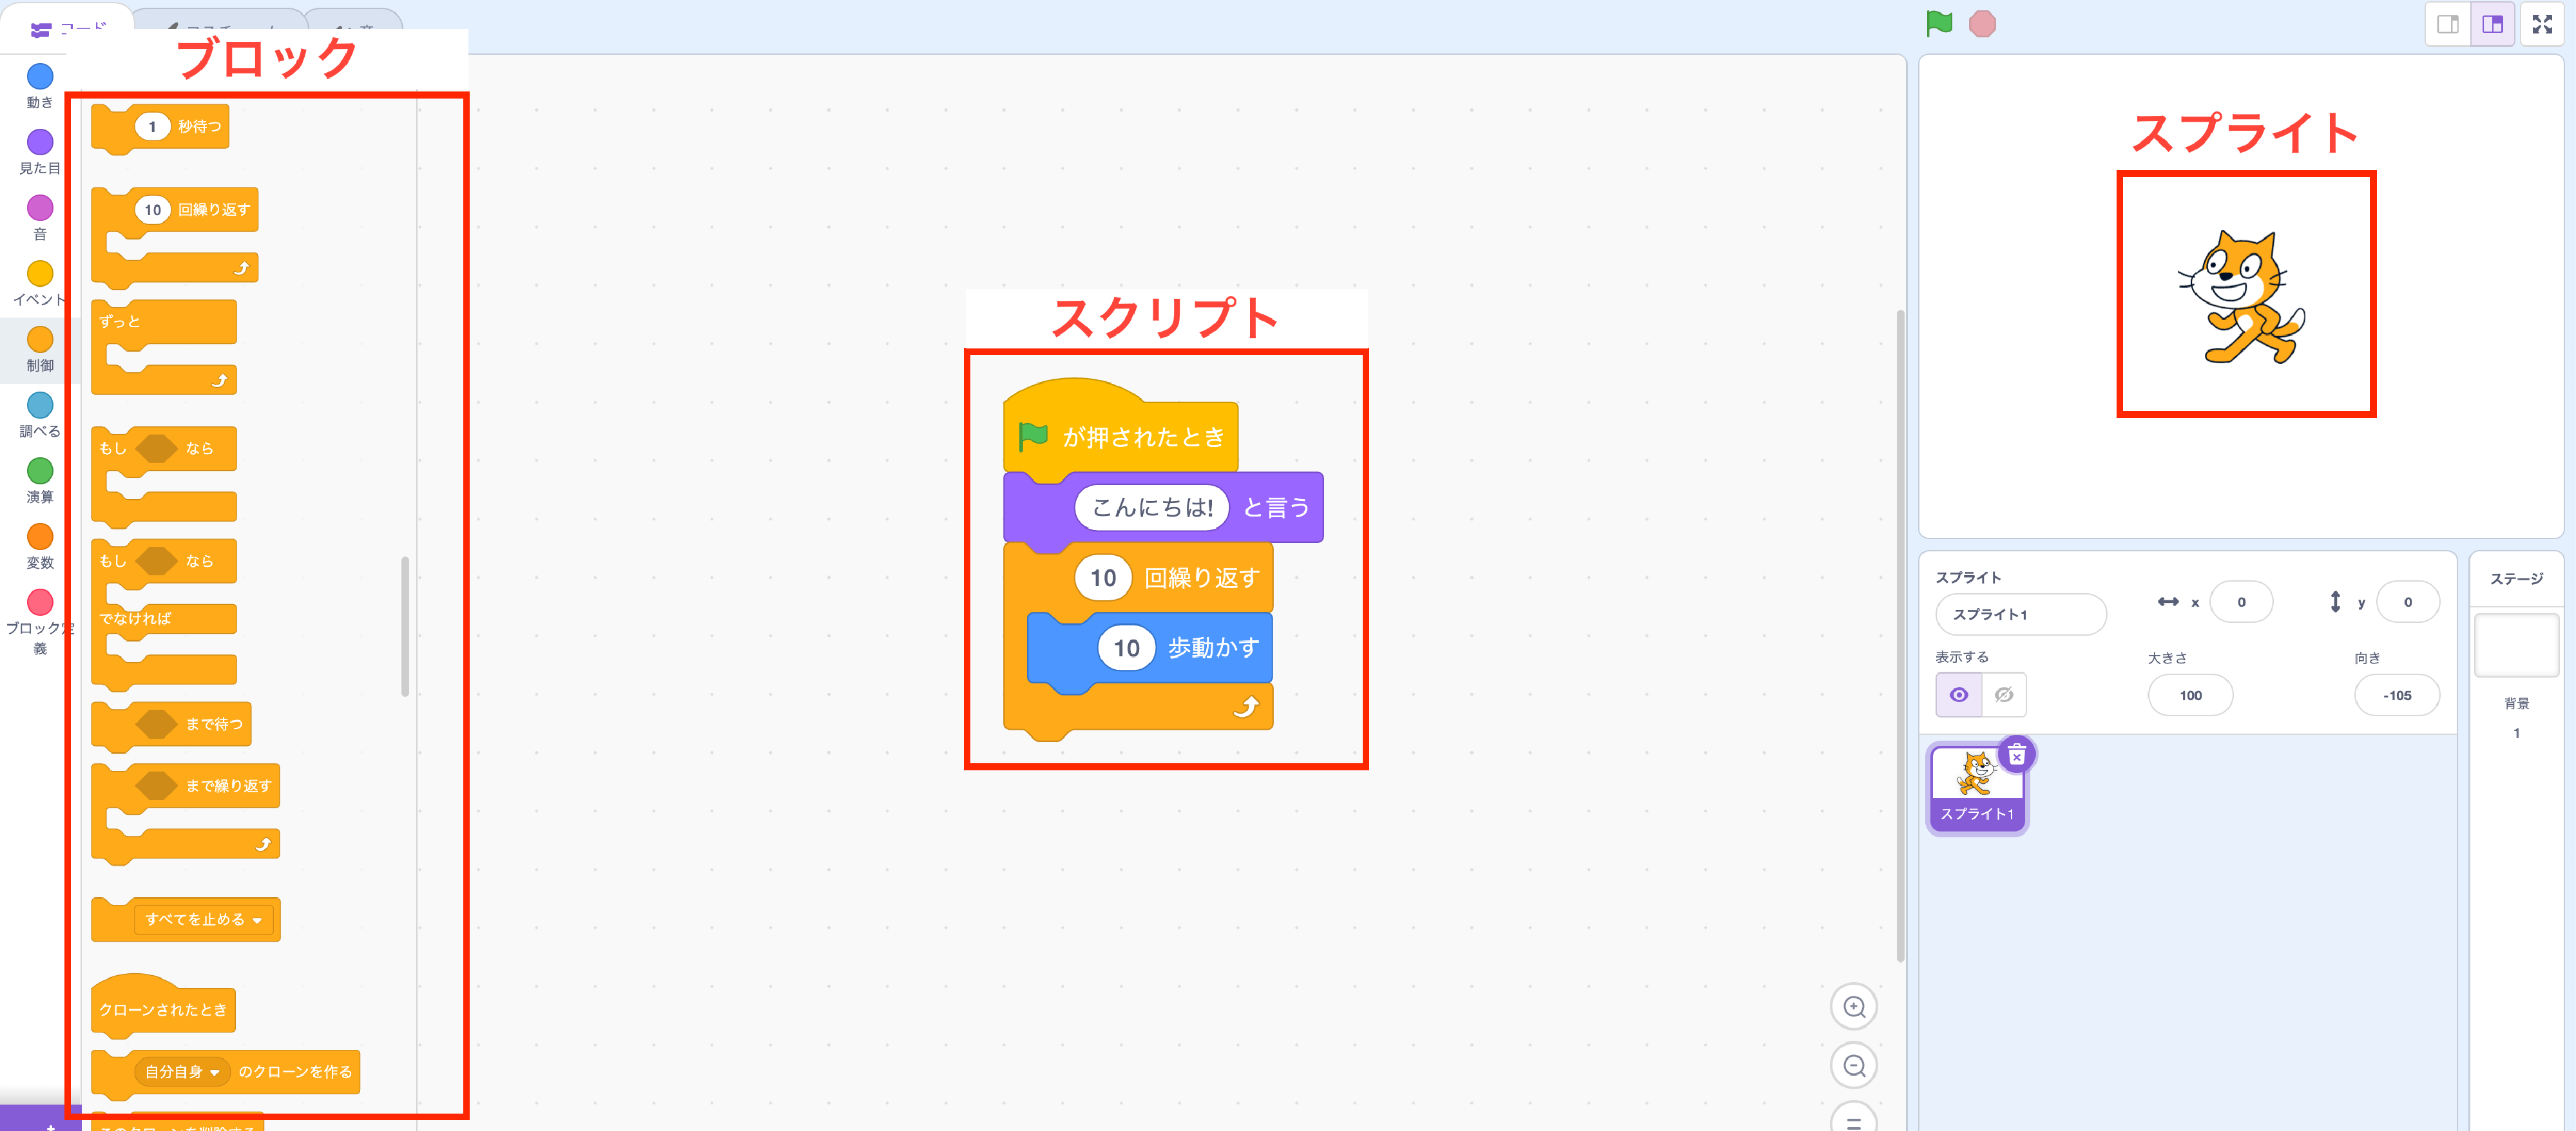
\includegraphics[width=0.9\linewidth]{Okamoto_fig/scratch-description.pdf}
	\caption{Scratchの作品制作画面}
	\label{fig:scratch-description}
\end{figure*}

\begin{figure*}[t]
	\centering
	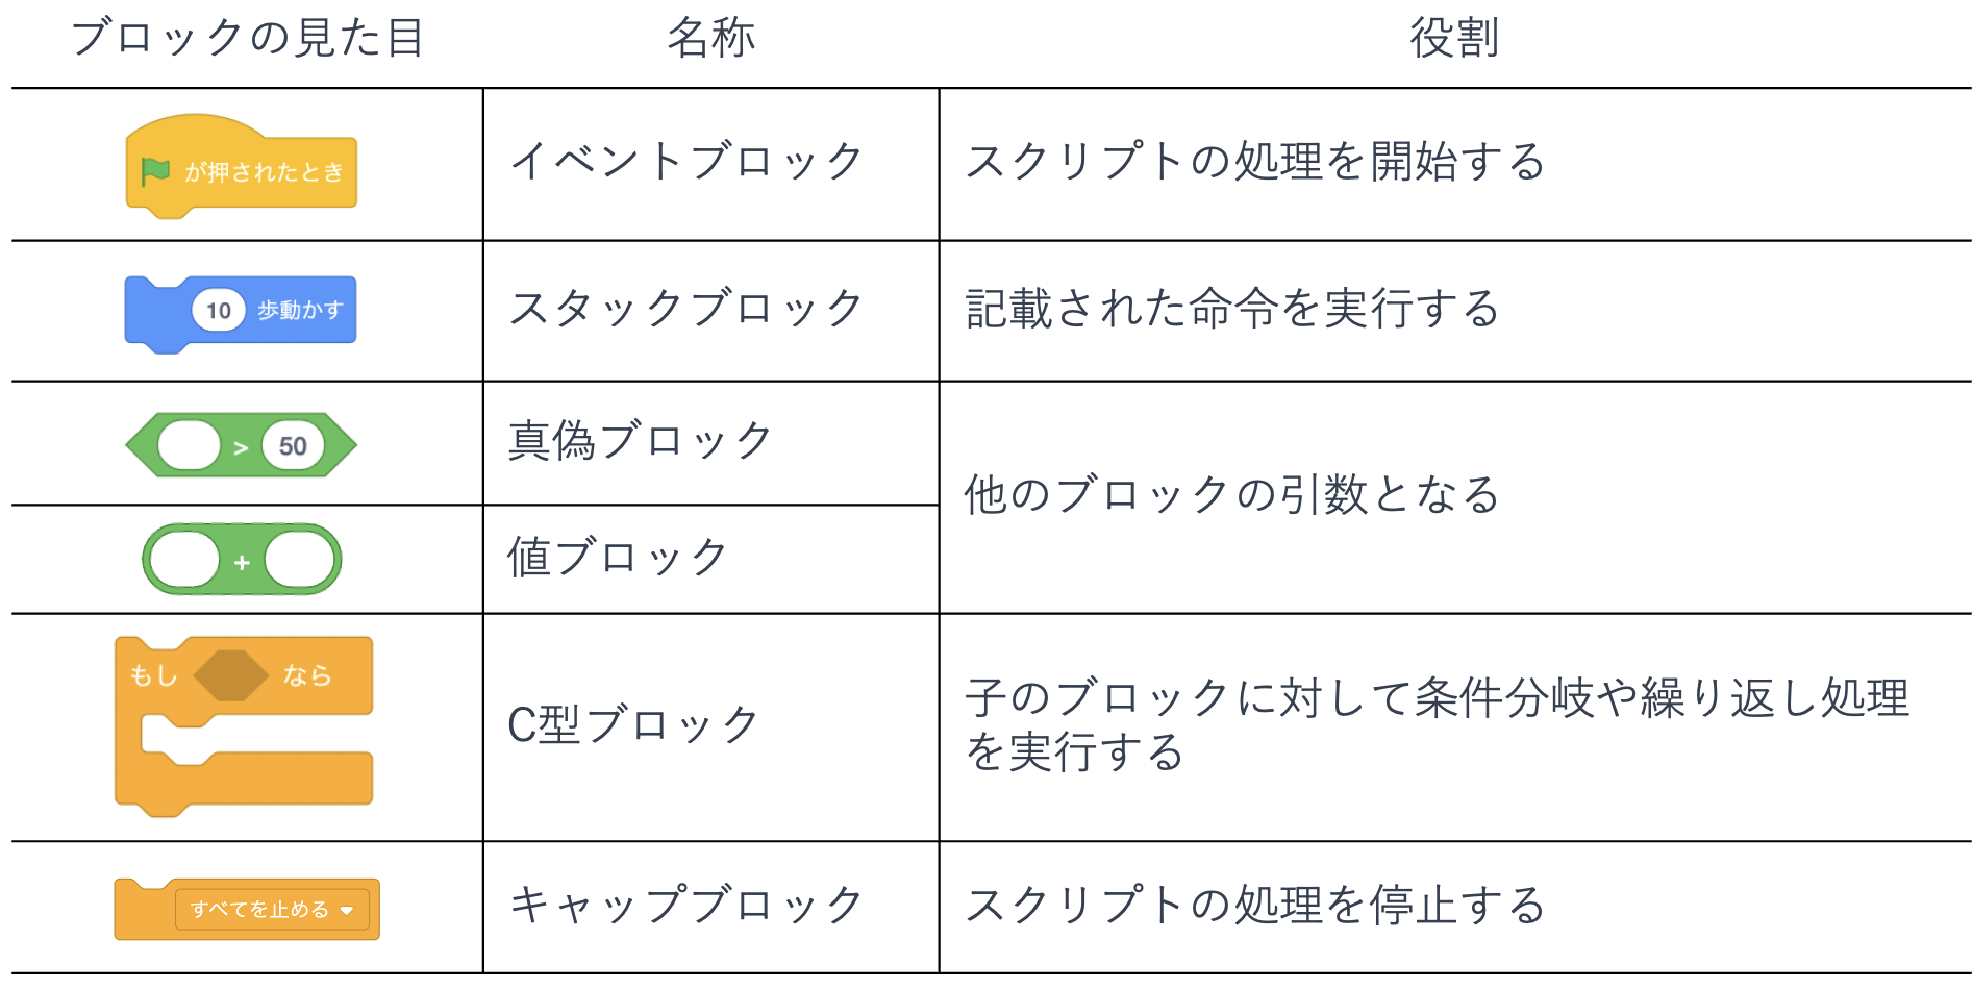
\includegraphics[width=0.9\linewidth]{Okamoto_fig/blocks.pdf}
	\caption{6種類のブロックとその性質}
	\label{fig:blocks}
\end{figure*}

\section{作品解析ツール:Dr.Scratch}
近年のプログラミング学習における学習者の目的の一つとして,コンピュテーショナルシンキング(CT)~\cite{Wing_2006}を身につけることが挙げられる.CTとはプログラミングの問題に対する抽象的な分析や,その問題を解決するための効率的な考え方の総称であり,主に問題を応用可能な一般式にする抽象化,問題を一般式に当てはめて表現する実装,問題を解いて確かめる分析の3手順の反復によって習熟していく.においてもプログラムの命令処理の結果がスプライトの動きとして出力されるため,作品制作のプログラム実装を通してCTを身につけることができる.しかし,ユーザが身につけたCTを把握するには,プログラムの実装内容を解析する必要があるため,プログラミング初学者にとって自身のCTを把握することは困難である.Scratchを用いたプログラミング学習を支援するツールとして,Morenoらはユーザが制作した作品に必要なCTを評価するDr.Scratch~\cite{Moreno_2015}を開発している.Dr.Scratchは,Scratch作品で利用されたブロックやプログラムの構造からCTスキルを計測し,7つの概念(CT7概念:抽象化,並列,論理,動機,フロー制御,ユーザ対話性,データ表現)で結果を出力する.表\ref{tab:analysis_method}に7概念の計測方法を示す.各CT概念は,作品中に使用されたブロックの種類やその数に基づいて,それぞれ0点から3点の4段階の点数によって評価される.また,作品自体はそれぞれのCT概念の点数を合計した0点から21点の22段階(CTスコア)で評価される.特に,CTスキルの区分としてCT習熟度が存在し,0点から7点をBasic,8点から14点をDeveloping,15点から21点をMasterとして3区分で評価している.

図\ref{fig:drscratch}はDr.Scartchによる作品の評価結果を示す.図\ref{fig:drscratch}には作品の制作にフロー制御,ユーザ対話性,データ表現が2点とそれ以外の概念が0点必要であると算出され,CTスコア合計点が6点として習熟度がBasicと評価している.このように,ユーザが制作した作品はDr.Scratchによって0点から3点のいずれかのCTスキルを獲得する.しかし,CT概念の一部は,同一概念に関わらず作品内で使用されるブロックの種類によって異なる点数を決定する.例えば.「同期」の概念では,待機ブロックを使用することで1点を獲得することができるが,メッセージブロックを使用してプログラムを停止する機能を実装する場合は2点を獲得する.したがって,本研究ではユーザのCTを明確に捉えるために,過去に制作した作品で使用する各CT概念の0点から3点までを区別して調査する.

\begin{table}[t]
    \caption{Dr.Scratchによる7つのCT概念の評価方法~\cite{Moreno_2015}}\label{tab:analysis_method}
    \centering
    \scalebox{0.6}{
        \begin{tabular}{|l|c|c|c|c}
            \hline
            \multicolumn{1}{|c|}{CT概念} & 1点 & 2点 & 3点 \\ \hline 
            抽象化 & \multicolumn{1}{c|}{2つ以上のスクリプトを使用} & \multicolumn{1}{c|}{定義ブロックを使用} & \multicolumn{1}{c|}{クローンブロックを使用} \\ \hline
            並列 & \begin{tabular}{c}緑の旗ブロックを2個以上使用\end{tabular} & \begin{tabular}{c}オブジェクトへのクリック動作により\\2つ以上のスクリプトを同時に\\実行する機能を実装\end{tabular} & \begin{tabular}{c}背景の切り替え,メッセージの受け取り\\など,イベント動作により2つ以上の\\スクリプトを同時に実行する機能を実装\end{tabular} \\ \hline
            論理 & Ifブロックを使用 & If elseブロックを使用 & 論理演算ブロックを使用 \\ \hline
            同期 & 待機ブロックを使用 & \begin{tabular}{c}メッセージを受信すると\\プログラムを停止する機能を実装\end{tabular} & \begin{tabular}{c}指定条件を満たすまで\\プログラムを停止する処理を実装\end{tabular} \\ \hline
            フロー制御 & 2個以上の処理ブロックを連結して使用 & \begin{tabular}{c}指定回数,または回数無制限の\\繰り返しブロックを使用\end{tabular} & 指定条件までの繰り返しブロックを使用 \\ \hline
            ユーザ対話性 & 緑の旗ブロックを使用 & \begin{tabular}{c}ユーザによる入力を伴うブロックを使用\end{tabular} & \begin{tabular}{c}マイクやビデオなど\\インタラクションを伴うブロックを使用\end{tabular} \\ \hline
            データ表現 & \begin{tabular}{c}オブジェクトの大きさや位置等の\\プロパティを編集\end{tabular} & 変数ブロックを使用 & リスト変数ブロックの使用 \\ \hline
        \end{tabular}
    }
\end{table}

\begin{figure*}[t]
	\centering
	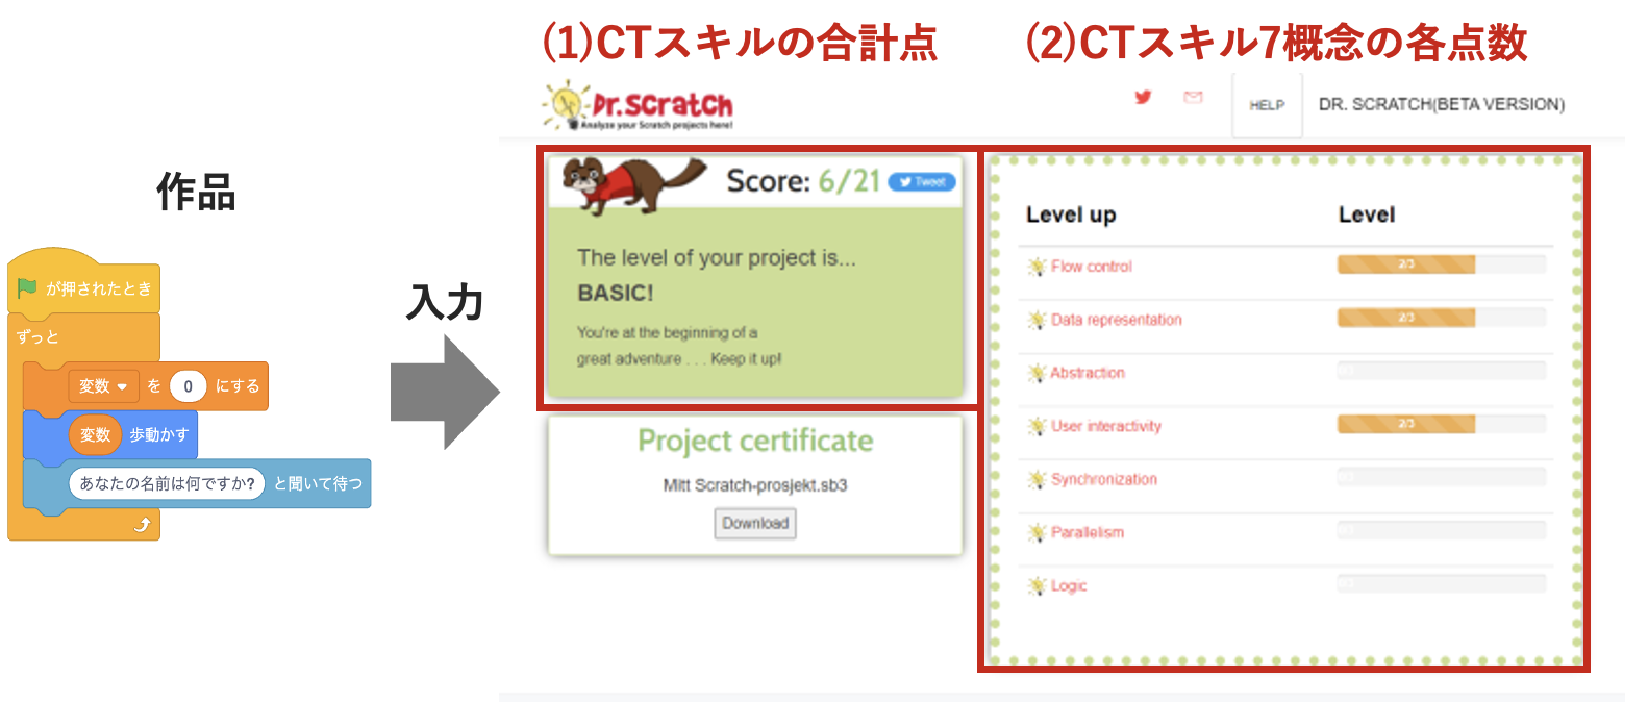
\includegraphics[width=1.0\linewidth]{Okamoto_fig/drscratch.pdf}
	\caption{Dr.Scratchの評価画面}
	\label{fig:drscratch}
\end{figure*}

\section{従来研究}
Scratchにおけるユーザのプログラミング能力の成長に関する研究として,Yangら~\cite{Yang_2015}はScratch
で50回以上の作品を制作したユーザ3,852人を対象に,作品制作回数の増加に伴うユーザが使用するブロックの種類数を調査している.その結果,ユーザは作品制作過程を経るごとに作品に使用するブロックの種類が増加し,リミックス(他のユーザの作品を再利用すること)の機能を用いているユーザほどその増加数が大きいことが明らかとなった.

Troianoら~\cite{Troiano_2019}は,13歳から14歳の生徒19人を対象に,それぞれの作品制作過程で作品に使用するCT概念を調査した.その結果,作品制作過程を経るごとに並列,論理,同期の点数が高くなる生徒が多いが,抽象化やデータ表現の点数が高くなる生徒が少ないことを示した.また,生徒が最終的に到達するCTスコアや,点数を伸ばすまでにかかる時間は,制作する作品のジャンル(シューティングゲームやアクションゲーム等)によって異なることを明らかにした.

安東ら~\cite{Ando_2021}はユーザのCTに合わせた作品推薦に向けて,ユーザが過去に制作した作品のCTスキルに基づいてユーザが次にCT習熟度が向上するかを予測する研究を行なった.

事前分析としてユーザがScratch上に公開している作品を収集し,各作品で使用されるCT概念をDr.Scratchを用いて計測し,ユーザが特定の習熟度に到達するまでに制作した作品の特徴を分析した.分析結果として,ユーザにとって習熟度DevelopingやMasterに分類されるオリジナル作品の制作は困難であり,ユーザは類似するCTスコアの作品を連続して制作することで習熟度が向上することが示唆された.特に,習熟度Developingのオリジナル作品を制作するまでに,ユーザは連続してBasicやDevelopingの作品を制作することが多く,Masterの作品を制作することは少ないことがわかり,習熟度Masterのオリジナル作品を制作するユーザの数は少なく,Masterの作品を連続して制作することは少ないことがわかった.

また,ユーザが過去に使用したCT概念に基づき,ユーザが次に制作する作品が次に制作する作品が当該習熟度以上の評価を得るかを予測モデルとして,事前分析の結果に基づき,目的変数の異なる2種類のモデルを構築した.

\begin{description}
\item [モデル1:]習熟度がDeveloping以上のオリジナル作品を制作するユーザを予測
\item [モデル2:]習熟度がMasterのオリジナル作品を制作するユーザを予測
\end{description}

説明変数としてはユーザが過去に作品制作で使用した7つのCT概念の0点から3点の獲得有無を用いた.モデルの構築にはランダムフォレストを用いており,事前分析で収集したデータを基に構築,予測を行った.結果としてDevelopingやMasterに到達するユーザと到達しないユーザの間では,過去に使用したCT概念に違いがあることが示唆された.

多くの従来研究では,Scratch上でユーザが制作する作品の特徴,または作品制作過程で使用するCT概念を調査しており,一部のCT概念の学習が困難であること,また特定の習熟度に到達するユーザとそうでないユーザ間では獲得したCT概念に違いがあることを明らかにしている.しかし,従来研究ではCT7概念の詳細な獲得過程については明らかになっていない.

安東らは,学習者のCT習熟度の把握を目的として,ScratchユーザのCT習熟度予測を行った.\todo{説明変数一緒で予測違うペアの統計}は従来研究における予測結果のうち,CTパス:ユーザが獲得してきたCT7概念が同じで,予測結果が異なる結果の数を示した表である.また,\todo{説明変数一緒でどっちも外れたやつ}は従来研究における予測結果のうち,CTパスが同じで,予測結果がどちらも外れた結果の数を示している.表1のモデル1では予測結果が異なる割合が多く,表2のモデル1では半分以上が予測結果が外れていることがわかる.
このことから,従来モデルではユーザのCT概念の獲得有無のみを説明変数としているため,ユーザのCT概念獲得過程は考慮されていないことが考えられる.しかし,実際にユーザは習熟度が向上するまでに様々な作品制作過程を確認している.

したがって,ユーザのCT7概念獲得過程に基づき,当該ユーザが保有するCTの習熟度の特定ができれば,Scratchにおけるユーザの作品制作過程に合わせた学習支援の役立てとなると期待する.


% \section{動機}
% 近年,プログラミング教育において学習者の成長過程を把握することは重要視されており,関連する研究が多数報告されている.Özgenら\todo{引用:Comparing Students’ Scratch Skills with Their Computational Thinking Skills in Terms of Different Variables}はScratchにおいて学習者がコンピュータの使用期間によってCTスコアが異ならないことを明らかにした.Ruijiaら\todo{引用:How Interest-Driven Content Creation Shapes Opportunities for Informal Learning in Scratch: A Case Study on Novices’ Use of Data Structures}はScratch上で公開されているプログラムを解析し,時間経過によって学習者がプログラムに変数やリストを使う数が増加することが明らかとなった.これらの研究では学習者のCTスキルの成長過程は分析,把握していない.しかし,プログラミング学習の目的はプログラムの実装方法の学習を通してCTを身につけることにあるため,教育者にとって学習者のCTスキルの成長過程を把握することは重要である.従来研究では学習者のCT習熟度の把握を目的として,ScratchユーザのCT習熟度予測を行った.\todo{説明変数一緒で予測違うペアの統計}は従来研究における予測結果のうち,CTパス:ユーザが獲得してきたCT7概念が同じで,予測結果が異なる結果の数を示した表である.また,\todo{説明変数一緒でどっちも外れたやつ}は従来研究における予測結果のうち,CTパスが同じで,予測結果がどちらも外れた結果の数を示している.表1のモデル1では予測結果が異なる割合が多く,表2のモデル1では半分以上が予測結果が外れていることがわかる.このことから,従来モデルではユーザのCTパスは考慮できておらず,精度が落ちてしまっていることが考えられる.

% 本研究では,ScratchユーザのCTスキルの成長過程の把握を目的として,続く\todo{次の章}で設定するリサーチクエスチョンに基づきScratchユーザのCT成長過程の分析を行い,次に学習者がCT習熟度が向上するかの到達予測を行う.本研究により,Scratchにおいてユーザの成長過程に合わせた学習支援の役立てとなることを期待する.


\section{リサーチクエスチョン(RQ)}
本章では目的達成のために設定したRQの動機について説明する.
\subsection{RQ1:CT習熟度が向上したユーザが獲得してきたCT7概念の違いはどの程度か?}
RQ1ではScratch作品の制作過程でCT習熟度が向上したユーザに着目して,各ユーザのCTパス:CT7概念の獲得過程の特徴量を分析する.本RQではCTパスの特徴量を分析することで,ユーザのCTパスの特徴,ユーザのCT概念の獲得過程に意味があるかを確認する.具体的には,ユーザのCT習熟度が向上する地点までの作品のCT7概念を計測し,CT習熟度が向上するまでに制作した作品数やCTパスの重複数を分析する.また,CTパス中に含まれるCT7概念にも着目し,成長過程によって用いられるCTスキルが異なるかどうかも確認する.詳しい内容については3章で説明する.
\subsection{RQ2:ユーザが獲得してきたCT7概念から次にCT習熟度が向上するかどうかを予測することは可能か?}
RQ2では学習者の成長過程によって到達習熟度が予測できるかを確認するため,ユーザのCTスコア獲得過程を説明変数として学習モデルを作成し,予測を行う.また,評価の際は従来モデルとの比較を行う.詳しい内容については4章で説明する.

\chapter{RQ1:CT習熟度が向上したユーザが獲得してきたCT7概念の違いはどの程度か?}\label{sec:chapter_3}
\section{概要}
本章では作品制作の過程でCT習熟度が向上したユーザに着目して,各ユーザが獲得してきたCT7概念の特徴を明らかにする.従来研究では,ユーザがCT習熟度が向上するまでにどのようなCTスキルを獲得してきているかは明らかにされていない.CT習熟度が向上したユーザが獲得してきたCT7概念の違いを明らかにするために,ユーザのCT習熟度が向上する地点までの作品のCT7概念を計測し,CT習熟度が向上するまでに制作した作品数や軌跡の重複数を調査する.
\section{データセット}\label{sec:chapter_3-1}
本研究では従来研究で収集された20件以上の作品を制作しているユーザの作品群を用いる.
Scratchは2019年1月3日に作品制作に使用可能な命令処理を一部追加,削除,名前の変更をする等,大規模なアップデートを実施しており,このアップデートに伴ってmicro:bitやLEGO MINDSTORMS 等の外部デバイスを用いた学習も行うことができるようになった.従来研究では,ユーザが共通の開発環境で制作した作品を比較するため,バージョン3.0をリリースした2019年1月3日から2020年1月3日までの間に初めて作品公開を行ったユーザを分析対象とし,サービス上に20件以上の作品を公開しているユーザ7,050人が制作した作品141,000件(7,050人×20件)を収集した.それらの作品をDr.ScratchによりCTスコアの計測を行い,失敗しなかった作品を制作したユーザ6,323人が1番目から20番目までに制作した作品126,460件を本分析の対象とする.
\section{分析手法}
データセットの中で,20番目の作品を制作するまでにBasicからDevelpingに向上したユーザ,DevelopingからMasterに向上したユーザを対象とし,向上したオリジナル作品からそれまでに獲得してきたCTスコアをJson形式で取得する.従来研究~\cite{Ando_2021}では,ユーザが特定の種類のブロックを1回でも使用すれば,そのブロックを学習したと捉えていることから,本論文でも同様にユーザが目標習熟度を満 たす作品を1回でも制作すれば当該習熟度に到達したと判断する.また,リミックス作品も学習の一部と考え,向上する過程でリミックス作品を含んでいる場合も取得する.

取得したCTスコアの軌跡から,向上するまでに制作した作品数,CTスコアの軌跡の重複数を計測する.
\section{分析結果}
\section{考察}

\chapter{RQ2:ユーザが獲得してきたCT7概念から次にCT習熟度が向上するかどうかを予測することは可能か?}
\section{CT習熟度到達タイミングの予測}
本章ではユーザが過去に使用したCT7概念の軌跡に基づいて,ユーザが次に制作する作品が当該習熟度以上の評価を得るかを予測するモデルとして,習熟度到達予測モデルを構築し,従来モデルとの比較を行う.また,評価結果をもとに,モデルの精度に寄与する要因について考察する.
\section{分析手法}
\subsection{CT習熟度到達予測モデルの構築}
従来研究より,目的変数の異なる2種類の予測モデルを構築する.

\begin{description}
\item [モデル1:]CTスコアが8点以上(Developing以上),のオリジナル作品を制作するユーザを予測
\item [モデル2:]CTスコアが15以上(Master),のオリジナル作品を制作するユーザを予測
\end{description}

目的変数は,{$N~(2 \leq N \leq 20)$}番目に目標習熟度に到達するオリジナル作品を制作したユーザを正例クラス,それ以外のユーザを負例クラスとする.例えば,モデル1の構築では2番目以降に制作するオリジナル作品でDeveloping以上の評価を得るユーザを正例クラスとし,そうでないユーザを負例クラスとして扱う.また従来研究~\cite{Ando_2021}では,ユーザが目標の習熟度を満たす作品を1回でも制作すれば当該習熟度に到達すると判断しているため,本研究でも同様に扱う.構築するモデルでは,ユーザがオリジナル作品で目標習熟度以上のCTスコア合計点を獲得した場合のみ到達したと判断し,リミックス作品によるCTスコア合計点の獲得は目標習熟度に到達したと判定しない.また,N=1となる正例クラスは,特徴量として説明する作品数が0件となるため,モデルの構築時には除外する.

説明変数には,\todo{ほげほげ}

モデルの構築には\ref{sec:chapter_3-1}節で収集したユーザ6,323人が1番目から20番目までに制作した作品126,460件を使用する.

\subsection{機械学習アルゴリズム}
本論文では,ユーザの作品制作過程に基づく習熟度到達予測モデルの構築にランダムフォレスト~\cite{Breiman_2001}を用いる.ランダムフォレストとは,与えられた学習のデータから複数の決定技を作成し,それらを組み合わせてモデルを構築するアンサンブル学習法である.図\ref{fig:random-forest}の概要図を示す.ランダムフォレストは,まず与えられた学習データからランダムに復元抽出を行い,N個分の学習データ群を生成し,各決定木で予測を行う.最後に各決定木で出力された結果を多数決することにより,分類を行う.

本論文では,Pythonのscikit-learnを用いてランダムフォレストの実装を行う.ランダムフォレストのパラメータは従来研究との比較を行うために,作成する決定木の個数(図\ref{fig:random-forest})は200個,各決定木の作成に使用する特徴量の個数は説明変数\todo{次元数}次元の平方根とする.また,表\ref{tab:user-class}は予測モデルの構築時に使用する正例クラスと負例クラスに該当するユーザの割合を示す.モデル1では正例クラスが3,436人.負例クラスが1,108人と正例クラスが負例クラスの約3倍の数存在し,モデル2でも正例クラスが1,345人,負例クラスが4,800人と負例クラスが正例クラスの約3倍存在することから, クラス間には偏りが存在しているといえる.したがって,モデル構築時に各クラスに出現する割合の逆数に基づいた重みづけを行う.例えば,モデル2では対象ユーザ6,145人のうち,正例クラスが3,436人,負例ユーザが1,108人存在するため,それぞれのクラスの事例に6,145 / 1,345 = 4.57, 6,145 / 4,800 = 1.28の重みを割り当てる.

\begin{figure*}[t]
	\centering
	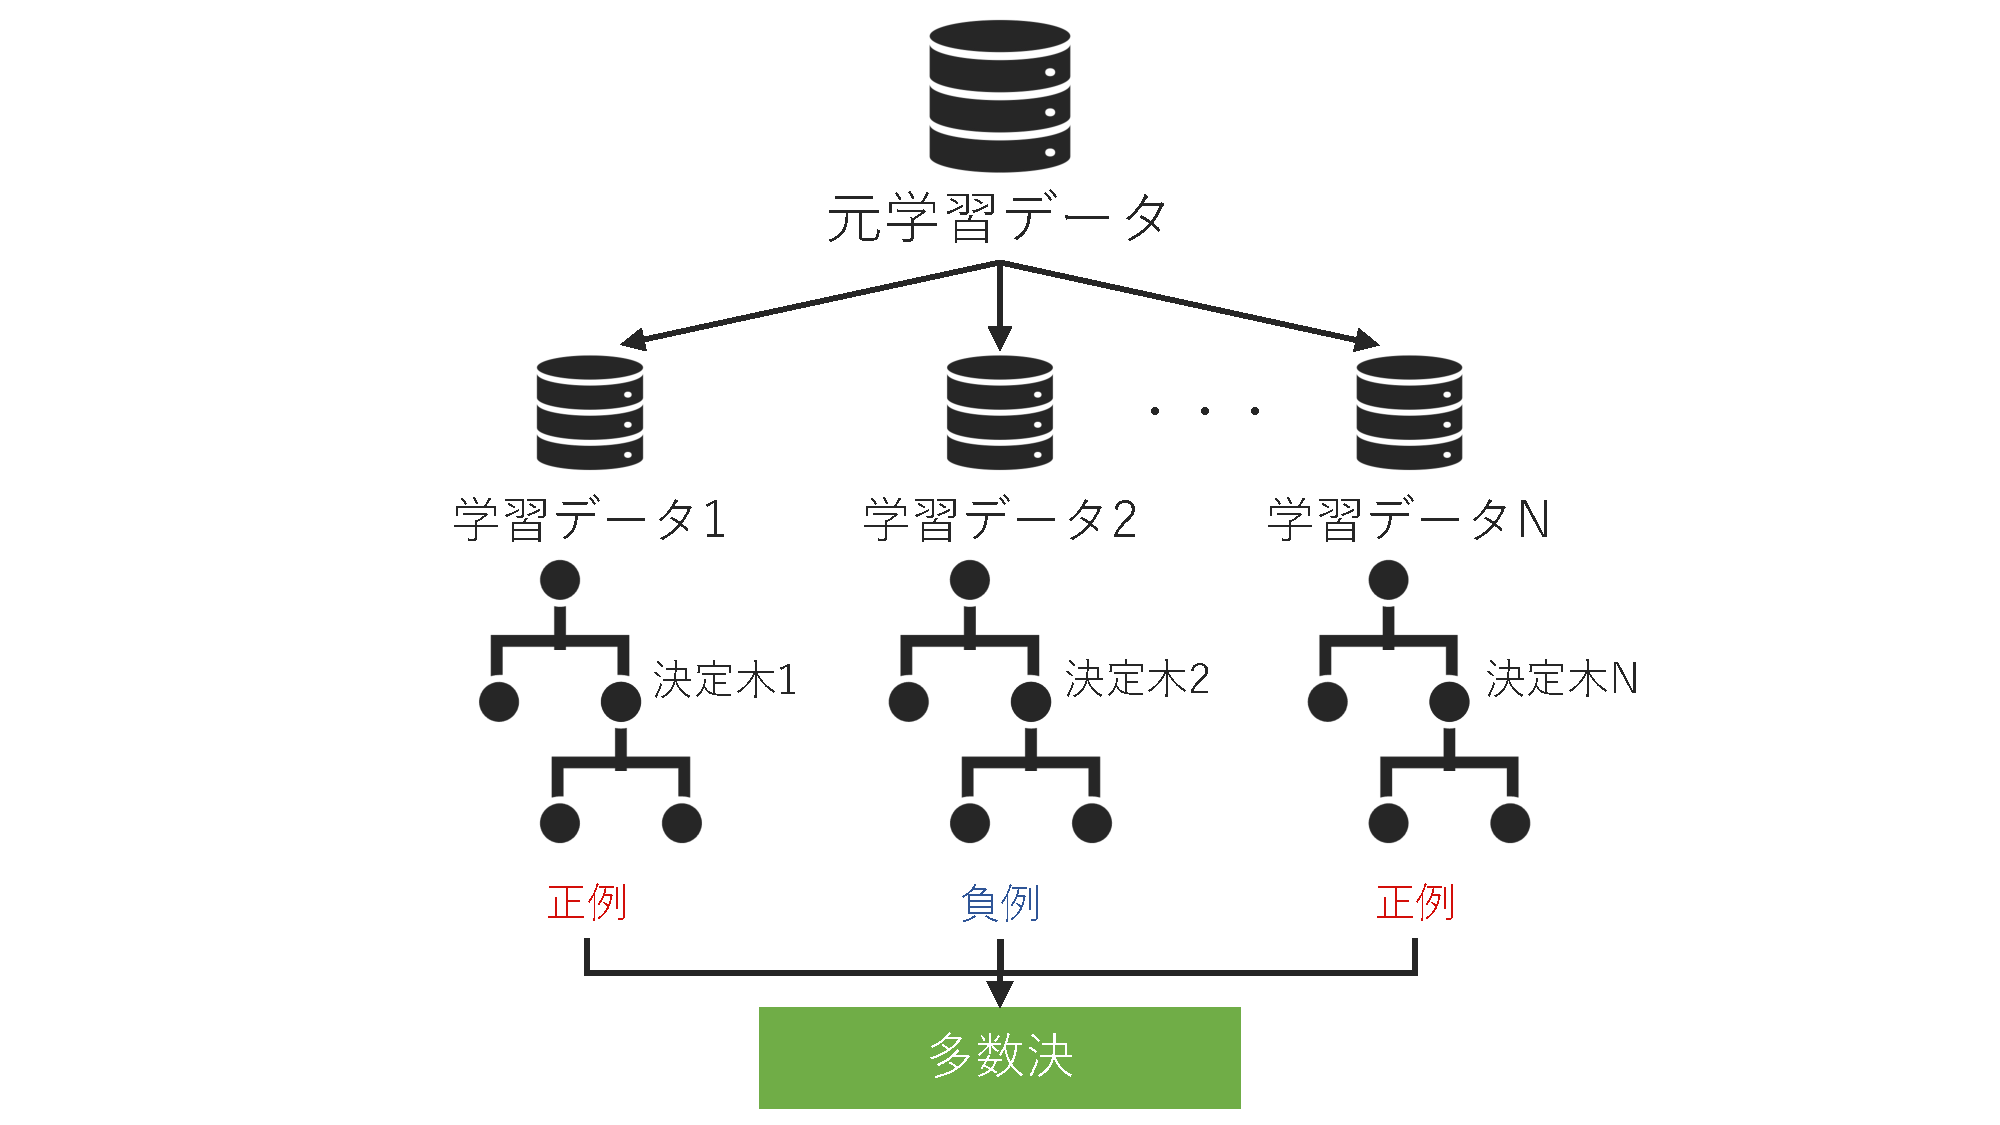
\includegraphics[width=1.0\linewidth]{Okamoto_fig/random-forest.pdf}
	\caption{ランダムフォレストの概略図}
	\label{fig:random-forest}
\end{figure*}

\begin{table}
  \caption{正例クラス,負例クラスに属するユーザ数の内訳}
  \label{tab:user-class}
  \centering
  \begin{tabular}{|c|c|c|}
    \hline
     & 正例クラス & 負例クラス\\
    \hline
    モデル1 & 3,436人 & 1,108人 \\
    \hline
    モデル2 & 1,345人 & 4,800人 \\
    \hline
  \end{tabular}
\end{table}

\subsection{モデルの評価方法}
本実験では,予測モデルの検証に従来研究と同じ層化K-分割交差検証を用いる.交差検証とは,モデルの構築時に使用するデータをK個に分割してK-1個を学習データ,残りの1個を検証データとして適用してK回繰り返すことで,予測モデルの汎化性能を評価する手法である.交差検証は,複数の学習データと検証データを組み合わせることで過学習(モデルが学習するデータには対応できるが,検証データには対応できない現象)の防止を実現する.

予測モデルの評価指標には適合率,再現率,F値を使用する.本研究で構築するモデルでは,ユーザが目標の習熟度に到達する(到達ユーザ)か到達していない(非到達ユーザ)かを予測するため,予測結果は以下の4つに分類できる.

\begin{description}
\item [True Positive(TP):]実際の到達ユーザに対して,到達ユーザであると正しく予測
\item [False Positive(FP):]実際の非到達ユーザに対して,到達ユーザであると誤って予測
\item [False Negative(FN):]実際の到達ユーザに対して,非到達ユーザであると誤って予測
\item [True Negative(TN):]実際の非到達ユーザに対して,非到達ユーザであると正しく予測
\end{description}

各評価指標は,上記の結果に基づいて算出される.適合率(Precision)は,式\ref{precision}に示すように予測モデルが到達ユーザと予測した内,実際に到達ユーザである割合を表す.

\begin{equation}
  適合率 = \frac{TP}{TP + FP} \label{precision}
\end{equation}
\vspace{.5mm}

再現率(Recall)は,式\ref{recall}で示すように到達ユーザの内,予測モデルにより正しく予測された到達ユーザの割合を表す.

\begin{equation}
  再現率 = \frac{TP}{TP + FN} \label{recall}
\end{equation}
\vspace{.5mm}

適合率と再現率は互いにトレードオフの関係にあるため,適合率,再現率の調和平均であるF値(F-measure)を用いる.F値は0から1の間の数値で算出され,値が高いほど予測モデルの精度が高いことを意味する.

\begin{equation}
  F値 = \frac{2 * 適合率 * 再現率}{適合率 + 再現率} \label{f-measure}
\end{equation}
\vspace{.5mm}

本研究では,交差検証によって10回の予測モデルの構築を行い,それぞれの予測結果で得られた3つの評価指標の平均値を算出し,評価を行う.

\section{実験結果}



\section{考察}

\chapter{妥当性への脅威}
\section{内的妥当性}
\section{外的妥当性}

\chapter{おわりに}


\chapter{タイトルページ,概要,目次}

{\bf 「和歌山大学システム工学部卒業論文/
大学院システム工学研究科修士論文用スタイルファイル」}\cite{wusethesis}
では,専用のタイトルページを出力する.
記述すべき項目は,
\begin{itemize}
  \item タイトル
  \item 著者名
  \item 学士(4年)/修士(M2)の設定
  \item 学科名/クラスタ名
  \item 学生番号
  \item 卒業年度
  \item 論文提出日
\end{itemize}
である.
これらのデータは,\verb|\maketitle|によってタイトルページに出力される.
また,概要の部分において,論文の内容をまとめる.その内容は論文の2ペー
ジ目(タイトルページの次)に出力される.
このソースでは,目次(\verb|\tableofcontents|)を出力している.
他に,図目次(\verb|\listoffigures|),表目次(\verb|\listoftables|)を
出力することもできるので,必要ならばそれぞれのコメントをはずす.
図目次,表目次については,第\ref{chap:fig-tab-exp}章において説明する.

\section{タイトル}
\subsection{title}
論文のタイトルを記述する.

\section{著者}
\subsection{author}
著者名を記述する.

\subsection{bachelar/master}
卒業論文の場合には,\verb|\master|をコメントアウトし,
\verb|\bachelar|を設定する.
修士論文の場合には,\verb|\bachelar|をコメントアウトし,
\verb|\master|を設定する.

\subsection{department}
所属を記述する.
システム工学科所属(学部生)の場合には``システム工'',
デザイン科学クラスタ所属(大学院生)の場合には``デザイン科学''と記述する.

\subsection{studentid}
学生番号を記述する.

\subsection{gyear}
卒業年度を記述する.

\section{提出日}
\subsection{date}
論文提出日を記述する.


\chapter{図,表,数式}\label{chap:fig-tab-exp}

論文では,図,表,数式などを効果的に使用する.

\section{図}

{\tt figure}環境を利用することによって図にキャプション
(\verb|\caption|)を付けることができる.図に付けられたキャプションは
\verb|\listoffigures|によって図目次として出力される.図には章ごとに通
し番号が付けられ,キャプションに\verb|\label|を設定しておくと,
``図\ref{fig:sample}''のように\verb|\ref|によって図を番号で参照するこ
とができる.図\ref{fig:sample}に{\tt figure}環境を用いた記述例を示す.

\begin{figure}
  \centering
    ここで図を取り込む.
    % 試しに,tiger.psが自分のマシンのどこに格納されているかを調べて
    % 以下の命令を有効にしてみて下さい.
    % ただし,同時に\begin{document}より前にある\usepackage{graphicx}
    % も有効にする必要があります.
    %\includegraphics[width=5cm,clip]{/usr/local/share/ghostscript/7.07/examples/tiger.ps}
  \caption{図の例}
  \label{fig:sample}
\end{figure}

また,{\tt graphicx.sty}などのスタイルファイルを利用することによって
EPS形式やPDF形式の図を文章の中に取り込むことができる.
この場合,\verb|\begin{document}|の前に\verb|\usepackage{graphicx}|を
追加する.

なお,図表の配置は基本的には\LaTeX{}が決めるので,思った位置に入らない
からといって無理に場所を指定するのはよくない.
どうしても位置を固定したい場合には,すべての文章が書きあがった後に指定
するとよい\footnote{そうしないと文章を書き換えるたびに,位置がずれる可能性がある}.

\section{表}

{\tt table}環境を利用することによって図と同じように,キャプションをつ
けたり,ラベルにより参照したりすることができる.また
\verb|\listoftables|によって表目次として出力される.
表\ref{tab:sample}に{\tt table}環境で作成した表を示す.

\begin{table}
  \caption{表の例}
  \label{tab:sample}
  \centering
  \begin{tabular}{|c|c|c|}
    \hline
    8 & 3 & 4\\
    \hline
    1 & 5 & 9 \\
    \hline
    6 & 7 & 2 \\
    \hline
  \end{tabular}
\end{table}

\section{数式}

\TeX では数式のための機能が豊富である.
{\tt equation}環境などを利用することによって数式に番号を付けることがで
きる.図や表と同じくラベルを付けておけば,``式\ref{exp:sample}''のよう
に数式を番号で参照することができる.

\begin{equation}
  y = ax^2 + bx + c \label{exp:sample}
\end{equation}

\chapter{参考文献}

文献を参照する場合には,論文の最後に参考文献として列挙するとともに,
\verb|\cite|を使って,例えば,
\begin{quote}
  文献\cite{latex}によれば…
\end{quote}
や,
\begin{quote}
  …である\cite{latex2e}.
\end{quote}
のように参照する.

文献の列挙には,{\tt thebibliography}環境などを用いる\footnote{使い方
は,この資料のソースを参照.}.

%%%%%%%%%%%%%%%%%%%%%%%%%%%%%%%%%%%%%%%%%%%%%%%%%%%%%%%%%%%%%%%%%%%%%%%%

%%
%% 謝辞
%%
%% \begin{acknowledgements}
%% 感謝します.
%% \end{acknowledgements}

%%%%%%%%%%%%%%%%%%%%%%%%%%%%%%%%%%%%%%%%%%%%%%%%%%%%%%%%%%%%%%%%%%%%%%%%

%%
%% 参考文献
%%

\bibliographystyle{junsrt}
\bibliography{Okamoto}

%%%%%%%%%%%%%%%%%%%%%%%%%%%%%%%%%%%%%%%%%%%%%%%%%%%%%%%%%%%%%%%%%%%%%%%%

%%
%% 付録
%%
% \appendix
% 
% \chapter{サンプルプログラム}
% 
% プログラムリストや実行結果など,本論を補足する上で必要と思われるものが
% あれば付録として付ける.
% 
% {
% \footnotesize
% \begin{verbatim}
% #include <stdio.h>
% int main(void)
% {
%     printf("Hello, World!\n");
%     return 0;
% }
% \end{verbatim}
% }

%%%%%%%%%%%%%%%%%%%%%%%%%%%%%%%%%%%%%%%%%%%%%%%%%%%%%%%%%%%%%%%%%%%%%%%%

\end{document}
